\documentclass[10pt]{opticajnl}
\journal{opticajournal} % use for journal or Optica Open submissions

% See template introduction for guidance on setting shortarticle option
\setboolean{shortarticle}{true}
% true = letter/tutorial
% false = research/review article

% ONLY applicable for journal submission shortarticle types:
% When \setboolean{shortarticle}{true}
% then \setboolean{memo}{true} will print "Memorandum" on title page header
% Otherwise header will remain as "Letter"
% \setboolean{memo}{true}
\usepackage{lineno}
\usepackage{listings}
\usepackage{color}  % Para colorear el código


\definecolor{dkgreen}{rgb}{0,0.6,0}
\definecolor{gray}{rgb}{0.5,0.5,0.5}
\definecolor{mauve}{rgb}{0.58,0,0.82}
\lstset{language=SQL,
  basicstyle={\small\ttfamily},
  belowskip=3mm,
  breakatwhitespace=true,
  breaklines=true,
  classoffset=0,
  columns=flexible,
  commentstyle=\color{dkgreen},
  framexleftmargin=0.25em,
  frameshape={}{yy}{}{}, %To remove to vertical lines on left, set `frameshape={}{}{}{}`
  keywordstyle=\color{blue},
  numbers=none, %If you want line numbers, set `numbers=left`
  numberstyle=\tiny\color{gray},
  showstringspaces=false,
  stringstyle=\color{dkgreen},
  tabsize=3,
  xleftmargin =1em
}

\lstdefinestyle{terminal}{
  backgroundcolor=\color{white},   % Fondo blanco
  basicstyle=\color{black}\ttfamily, % Texto negro en fuente monoespaciada
  keywordstyle=\color{black}\bfseries, % Palabras clave en azul y negrita
  commentstyle=\color{black}\ttfamily, % Comentarios en verde
  stringstyle=\color{black}\ttfamily, % Cadenas en rojo
  morekeywords={sudo, apt-get, install, cd, ls, mkdir, rm, rmdir, cp, mv, echo, cat, nano, vim, grep, find, chmod, chown, systemctl, service, update, upgrade, reboot, shutdown, exit}, % Comandos comunes de terminal
  breaklines=true, % Permitir saltos de línea
  frame=single, % Marco alrededor del código
  framerule=0.5pt, % Grosor del marco
  rulecolor=\color{gray}, % Color del marco
  xleftmargin=0.05\textwidth, % Margen izquierdo
  xrightmargin=0.05\textwidth, % Margen derecho
  aboveskip=1em, % Espacio antes del bloque de código
  belowskip=1em % Espacio después del bloque de código
}


%\linenumbers % Turn off line numbering for Optica Open preprint submissions.

\title{Trabajo de prácticas BDGE}

\author[1,2,3]{Luis Ardévol Mesa, Miguel Mato Martínez}


\begin{abstract}
Usando una conjunto de datos de partidos de tenis, se usarán distintos tipos de base de datos para realizar consultas acerca de los mismos. En concreto, se tratarán bases de datos relaciones y con datos agregados en PostgreSQL, bases de datos distribuidas con SQL usando CITUS Data, y dos tipos de bases de datos noSQL: documentales con MongoDB y en grafo con Neo4j.
\end{abstract}

\setboolean{displaycopyright}{false} % Do not include copyright or licensing information in submission.

\begin{document}

\maketitle

\section{Bases de datos relacionales (PostgreSQL)}

\begin{figure}[H]
  \centering
  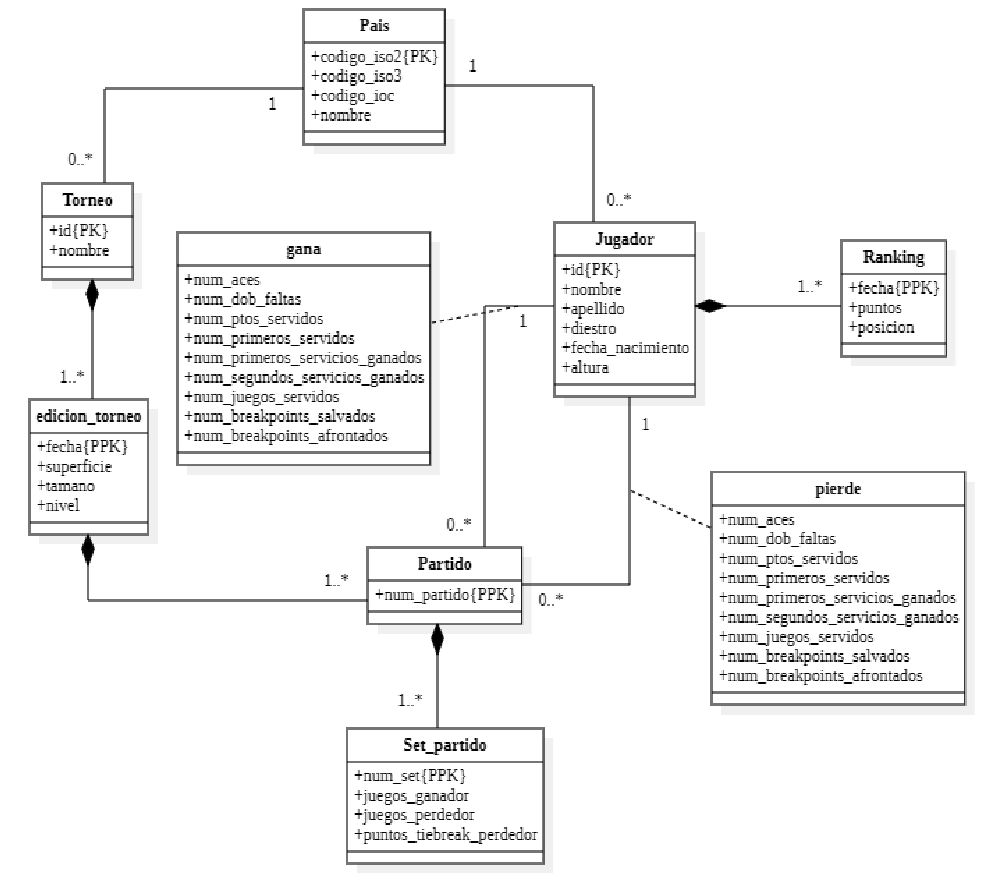
\includegraphics[width=0.7\textwidth]{fotos/esquema.png}
  \caption{Esquema de la base de datos de partidos de tenis.}
  \label{fig:schbd}
\end{figure}

\begin{lstlisting}[style=terminal]
psql -U alumnogreibd -d tenis -f /home/alumnogreibd/BDGE/datos/datos_tenis/schema.sql
\end{lstlisting}

\begin{lstlisting}[style=terminal]
psql -U alumnogreibd -d tenis -c "\copy pais from /home/alumnogreibd/BDGE/datos/datos_tenis/pais.csv csv"
psql -U alumnogreibd -d tenis -c "\copy jugador from /home/alumnogreibd/BDGE/datos/datos_tenis/jugador.csv csv"
psql -U alumnogreibd -d tenis -c "\copy torneo from /home/alumnogreibd/BDGE/datos/datos_tenis/torneo.csv csv"
psql -U alumnogreibd -d tenis -c "\copy edicion_torneo from /home/alumnogreibd/BDGE/datos/datos_tenis/edicion_torneo.csv csv"
psql -U alumnogreibd -d tenis -c "\copy partido from /home/alumnogreibd/BDGE/datos/datos_tenis/partido.csv csv"
psql -U alumnogreibd -d tenis -c "\copy sets_partido from /home/alumnogreibd/BDGE/datos/datos_tenis/sets_partido.csv csv"
psql -U alumnogreibd -d tenis -c "\copy ranking from /home/alumnogreibd/BDGE/datos/datos_tenis/ranking.csv csv"
\end{lstlisting}



\subsubsection{Muestra todos los ganadores del torneo "Wimbledon" (Nombre apellidos y año). Ordena el resultado por año.}

\begin{lstlisting}[language=SQL]
select j.nombre, j.apellido, extract(year from p.fecha) as ano
from jugador j, partido p, torneo t
where j.id = p.ganador 
  and t.id = p.torneo 
  and t.nombre = 'Wimbledon' 
  and p.ronda = 'F'
order by ano
\end{lstlisting}


\subsubsection{Muestra los años en los que Roger Federer ganó algún torneo de nivel Gran Slam (G) o Master 1000 (M). Para cada año, muestra el número de torneos y lista sus nombres (ordenados por la fecha de celebración). Ordena el resultado por el año}

\begin{lstlisting}[language=SQL]
select extract(year from et.fecha) as ano, count(distinct t.id) as numero_torneos, string_agg(t.nombre, ', ' order by et.fecha) as torneos
from jugador j, partido p, torneo t, edicion_torneo et
where j.id = p.ganador
  and t.id = et.torneo
  and p.torneo = t.id
  and p.fecha = et.fecha
  and p.ronda = 'F'
  and j.nombre = 'Roger'
  and j.apellido = 'Federer'
  and et.nivel in ('G', 'M')
group by ano
\end{lstlisting}

\subsubsection{Muestra los partidos de semifinales (ronda='SF') y final (ronda = 'F') del torneo de "Roland Garros" del 2018. Para cada partido muestra la ronda, el tipo de desenlace, el nombre y apellidos del ganador y el nombre y apellidos del perdedor y el resultado con el número de juegos del ganador y del perdedor en cada set, y opcionalmente en paréntesis el número de juegos del perdedor en el tie break}

\begin{lstlisting}[language=SQL]
select p.ronda, p.desenlace, jg.nombre || ' ' || jg.apellido AS ganador, jp.nombre || ' ' || jp.apellido AS perdedor, STRING_AGG(sp.juegos_ganador || '-' || sp.juegos_perdedor ||
      case
          when sp.puntos_tiebreak_perdedor is not null then
              '(' || sp.puntos_tiebreak_perdedor || ')'
          else
              ''
      end, ', ' order by sp.num_set) as resultado
from partido p, jugador jg, jugador jp, sets_partido sp, torneo t
where jg.id = p.ganador
  and jp.id = p.perdedor
  and p.fecha = sp.fecha
  and p.num_partido = sp.num_partido
  and t.id = p.torneo
  and p.ronda in ('SF', 'F')
  and t.nombre = 'Roland Garros'
  and extract(year from p.fecha) = '2018'
group by p.ronda, p.desenlace, jg.nombre, jg.apellido, jp.nombre, jp.apellido, p.fecha
\end{lstlisting}

\subsubsection{Muestra la lista de jugadores españoles (ES) que ganaron algún torneo de nivel Gran Slam (G). Para cada jugador muestra los siguientes datos resumen de todos sus partidos: número de partidos jugados, porcentaje de victorias, porcentaje de aces, porcentaje de dobles faltas, porcentaje de servicios ganados, porcentaje de restos ganados, porcentaje de break points salvados (de los sufridos en contra), porcentaje de break points ganados (de los provocados a favor)}

\begin{lstlisting}[language=SQL]
with jugadores_espanoles_ganadores as (
    select distinct j.id as id_jugador, j.nombre || ' ' || j.apellido as jugador
    from partido p, jugador j, edicion_torneo et 
    where p.ganador = j.id 
        and p.torneo = et.torneo 
        and p.fecha = et.fecha
        and j.pais = 'ES'
        and p.ronda = 'F'
        and et.nivel = 'G'
)

select jeg.jugador, count(p.num_partido) as partidos,
    round(100.0 * sum(case when jeg.id_jugador = p.ganador then 1 else 0 end) / count(p.num_partido), 1) as pcje_victorias, 
    round(100.0 * sum(case when jeg.id_jugador = p.ganador then p.num_aces_ganador else p.num_aces_perdedor end) / 
        nullif(sum(case when jeg.id_jugador = p.ganador then p.num_ptos_servidos_ganador  else p.num_ptos_servidos_perdedor end), 0), 1) as pcje_aces, 
    round(100.0 * sum(case when jeg.id_jugador = p.ganador then p.num_dob_faltas_ganador  else p.num_dob_faltas_perdedor  end) / 
        nullif(sum(case when jeg.id_jugador = p.ganador then p.num_ptos_servidos_ganador  else p.num_ptos_servidos_perdedor end), 0), 1) as pcje_dobles_faltas, 
    round(100.0 * sum(case when jeg.id_jugador = p.ganador then p.num_primeros_servicios_ganados_ganador + p.num_segundos_servicios_ganados_ganador 
            else p.num_primeros_servicios_ganados_perdedor + p.num_segundos_servicios_ganados_perdedor end) / 
        nullif(sum(case when jeg.id_jugador = p.ganador then p.num_ptos_servidos_ganador  else p.num_ptos_servidos_perdedor end), 0), 1) as pcje_servicios_ganados, 
    round(100.0 * sum(case when jeg.id_jugador = p.ganador 
            then p.num_ptos_servidos_perdedor - p.num_primeros_servicios_ganados_perdedor - p.num_segundos_servicios_ganados_perdedor 
            else p.num_ptos_servidos_ganador - p.num_primeros_servicios_ganados_ganador - p.num_segundos_servicios_ganados_ganador end) / 
        nullif(sum(case when jeg.id_jugador = p.ganador then p.num_ptos_servidos_perdedor else p.num_ptos_servidos_ganador end), 0), 1) as pcje_restos_ganados,
    round(100.0 * sum(case when jeg.id_jugador = p.ganador then p.num_break_salvados_ganador else p.num_break_salvados_perdedor end) / 
        nullif(sum(case when jeg.id_jugador = p.ganador then p.num_break_afrontados_ganador else p.num_break_afrontados_perdedor end), 0), 1) as pcje_breaks_salvados, 
    round(100.0 * sum(case when jeg.id_jugador = p.ganador then p.num_break_afrontados_perdedor - p.num_break_salvados_perdedor 
            else p.num_break_afrontados_ganador - p.num_break_salvados_ganador end) / 
        nullif(sum(case when jeg.id_jugador = p.ganador then p.num_break_afrontados_perdedor else p.num_break_afrontados_ganador end), 0), 1) as pcje_breaks_ganados
from jugadores_espanoles_ganadores jeg, partido p
where jeg.id_jugador = p.ganador 
	or jeg.id_jugador = p.perdedor
group by jeg.jugador
\end{lstlisting}

\subsubsection{Lista los jugadores que fueron derrotados (en algún partido del 2018) por el rival de Rafael Nadal de la primera ronda (R128) de Roland Garros de 2018}

\begin{lstlisting}[language=SQL]
with rival_nadal as (
	select case when jg.nombre = 'Rafael' then jp.id else jg.id end as id_jugador, 
		case when jg.nombre = 'Rafael' then jp.nombre || ' ' || jp.apellido else jg.nombre || ' ' || jg.apellido end as jugador
	from partido p, jugador jg, jugador jp, edicion_torneo et, torneo t 
	where p.ganador = jg.id 
		and p.perdedor = jp.id
		and p.torneo = et.torneo 
		and p.fecha = et.fecha
		and et.torneo = t.id 
		and t.nombre = 'Roland Garros'
		and p.ronda = 'R128'
		and extract(year from p.fecha) = '2018'
		and (jg.nombre = 'Rafael' and jg.apellido = 'Nadal' or jp.nombre = 'Rafael' and jp.apellido = 'Nadal') 
)

select j.nombre || ' ' || j.apellido as jugador, j.pais as pais
from rival_nadal rn, partido p, jugador j
where rn.id_jugador = p.ganador 
	and p.perdedor = j.id
	and extract(year from p.fecha) = '2018'
\end{lstlisting}


































\section{Datos agregados en SQL (PostgreSQL)}
(un array es homogeneo, una tupla no !!)

\subsection{Tipos compuestos}

\begin{lstlisting}[language=SQL]
create type pais_info as (
	codigo_iso2 char(2),
	codigo_iso3 char(3),
	codigo_ioc char(3),
	nombre varchar(100)
)

create type torneo_info as (
	id integer,
	nombre varchar(100),
	pais pais_info
)

create type edicion_torneo_info as (
	torneo torneo_info,
	fecha date,
	superficie varchar(20),
	tamano integer,
	nivel char(1)
)

create type set_info as (
	torneo torneo_info, --quitar
	fecha date, --quitar
	num_partido integer, --quitar
    num_set integer,
   juegos_ganador integer,
   juegos_perdedor integer,
   puntos_tiebreak_perdedor integer
)

create type jugador_stats as (
	num_aces integer,
	num_dob_faltas integer,
	num_ptos_servidos integer,
	num_primeros_servicios integer,
	num_primeros_servicios_ganados integer,
	num_segundos_servicios_ganados integer,
	num_juegos_servidos integer,
	num_break_salvados integer,
	num_break_afrontados integer
)

create type jugador_info as (
   id integer,
   nombre varchar(100),
   apellido varchar(100),
   diesto boolean,
   fecha_nacimiento date,
   pais pais_info,
   altura integer
)
\end{lstlisting}

\begin{lstlisting}[language=SQL]
create table partidos (
  torneo edicion_torneo_info,
  fecha date,
  num_partido integer,
  num_sets integer,
  info_sets set_info array, -- array de elementos de tipo set_info
  ronda varchar(5), 
	desenlace char(1), 
	ganador jugador_info,
	perdedor jugador_info,
	ganador_stats jugador_stats,
	perdedor_stats jugador_stats
)
\end{lstlisting}

\begin{lstlisting}[language=SQL]
insert into partidos(
torneo, fecha, num_partido, num_sets, info_sets, ronda, desenlace, ganador, perdedor, ganador_stats, perdedor_stats)
select
   -- campo 'torneo' (tipo 'torneo_info')
   case
       when t.id is null then null
       else cast((cast((t.id, t.nombre, cast((pa.codigo_iso2, pa.codigo_iso3, pa.codigo_ioc, pa.nombre) as pais_info)) as torneo_info), 
       et.fecha, et.superficie, et.tamano, et.nivel) as edicion_torneo_info)
   end as torneo,
  
   p.fecha as fecha,
   p.num_partido as num_partido,
   p.num_sets as num_sets,
  
   -- campo 'info_set' (array de 'set_info')
   array(select cast((cast((t.id, t.nombre, cast((pa.codigo_iso2, pa.codigo_iso3, pa.codigo_ioc, pa.nombre) as pais_info)) as torneo_info),
                      sp.fecha, sp.num_partido, sp.num_set, sp.juegos_ganador, sp.juegos_perdedor, sp.puntos_tiebreak_perdedor) as set_info)
         from public.sets_partido sp
         where sp.torneo = p.torneo
         	and sp.fecha = p.fecha
         	and sp.num_partido = p.num_partido
         order by sp.num_set) as info_sets,
  
   p.ronda as ronda,
   p.desenlace as desenlace,
  
   -- campo 'ganador' (tipo 'jugador_info')
   case
       when jg.id is null then null
       else cast((jg.id, jg.nombre, jg.apellido, jg.diestro, jg.fecha_nacimiento,
       		   cast((pg.codigo_iso2, pg.codigo_iso3, pg.codigo_ioc, pg.nombre) as pais_info),
       		   jg.altura) as jugador_info)
   end as ganador,
  
   -- campo 'perdedor' (tipo 'jugador_info')
   case
       when jp.id is null then null
       else cast((jp.id, jp.nombre, jp.apellido, jp.diestro, jp.fecha_nacimiento,
       		   cast((pp.codigo_iso2, pp.codigo_iso3, pp.codigo_ioc, pp.nombre) as pais_info),
       		   jp.altura) as jugador_info)
   end as perdedor,
  
   -- campo 'ganador_stats' (tipo 'jugador_stats')
   case
       when jg.id is null and jp.id is null then null
       else cast((p.num_aces_ganador, p.num_dob_faltas_ganador,
           	   p.num_ptos_servidos_ganador, p.num_primeros_servicios_ganador,
           	   p.num_primeros_servicios_ganados_ganador, p.num_segundos_servicios_ganados_ganador,
           	   p.num_juegos_servidos_ganador, p.num_break_salvados_ganador,
           	   p.num_break_afrontados_ganador) as jugador_stats)
   end as ganador_stats,
  
   -- campo 'perdedor_stats' (tipo 'jugador_stats')
   case
       when jg.id is null and jp.id is null then null
       else cast((p.num_aces_perdedor, p.num_dob_faltas_perdedor,
           	   p.num_ptos_servidos_perdedor, p.num_primeros_servicios_perdedor,
           	   p.num_primeros_servicios_ganados_perdedor, p.num_segundos_servicios_ganados_perdedor,
           	   p.num_juegos_servidos_perdedor, p.num_break_salvados_perdedor,
           	   p.num_break_afrontados_perdedor) as jugador_stats)
   end as perdedor_stats
from public.partido p join public.edicion_torneo et on et.fecha = p.fecha and et.torneo = p.torneo 
	left join public.torneo t on t.id = et.torneo
	left join public.pais pa on t.pais = pa.codigo_iso2
	left join public.jugador jg on p.ganador = jg.id
	left join public.pais pg on jg.pais = pg.codigo_iso2
	left join public.jugador jp on p.perdedor = jp.id
	left join public.pais pp on jp.pais = pp.codigo_iso2
\end{lstlisting}





\subsubsection{Muestra todos los ganadores del torneo ``Wimbledon'' (Nombre apellidos y año). Ordena el resultado por año.}

\begin{lstlisting}[language=SQL]
select (ganador).nombre, (ganador).apellido, extract(year from fecha) as ano
from partidos
where (torneo).torneo.nombre = 'Wimbledon'
	and ronda = 'F'
order by ano
\end{lstlisting}





\subsubsection{Muestra los años en los que Roger Federer ganó algún torneo de nivel Gran Slam (G) o Master 1000 (M). Para cada año, muestra el número de torneos y lista sus nombres (ordenados por la fecha de celebración). Ordena el resultado por el año}

\begin{lstlisting}[language=SQL]
select extract(year from (torneo).fecha) as ano, count(distinct (torneo).torneo.id) as numero_torneos, 
	string_agg((torneo).torneo.nombre, ', ' order by (torneo).fecha) as torneos
from partidos
where (torneo).nivel in ('G', 'M')
	and (ganador).nombre = 'Roger'
	and (ganador).apellido = 'Federer'
	and ronda = 'F'
group by ano
\end{lstlisting}





\subsubsection{Muestra los partidos de semifinales (ronda='SF') y final (ronda = 'F') del torneo de "Roland Garros" del 2018. Para cada partido muestra la ronda, el tipo de desenlace, el nombre y apellidos del ganador y el nombre y apellidos del perdedor y el resultado con el número de juegos del ganador y del perdedor en cada set, y opcionalmente en paréntesis el número de juegos del perdedor en el tie break}

\begin{lstlisting}[language=SQL]
select ronda, desenlace, 
	(ganador).nombre || ' ' || (ganador).apellido as ganador,
	(perdedor).nombre || ' ' || (perdedor).apellido as perdedor, 
	(select string_agg(iset.juegos_ganador || '-' || iset.juegos_perdedor ||
	case
		when iset.puntos_tiebreak_perdedor is not null then 
			'(' || iset.puntos_tiebreak_perdedor || ')'
		else ''
	end, ', ' order by iset.num_set) 
	from unnest(info_sets) as iset) as resultado
from partidos
where ronda in ('SF', 'F')
	and (torneo).torneo.nombre = 'Roland Garros'
	and extract(year from fecha) = '2018'
\end{lstlisting}





\subsubsection{Muestra la lista de jugadores españoles (ES) que ganaron algún torneo de nivel Gran Slam (G). Para cada jugador muestra los siguientes datos resumen de todos sus partidos: número de partidos jugados, porcentaje de victorias, porcentaje de aces, porcentaje de dobles faltas, porcentaje de servicios ganados, porcentaje de restos ganados, porcentaje de break points salvados (de los sufridos en contra), porcentaje de break points ganados (de los provocados a favor)}

\begin{lstlisting}[language=SQL]
with jugadores_espanoles_ganadores as (
    select distinct (ganador).id as id_jugador, (ganador).nombre || ' ' || (ganador).apellido AS jugador
    from partidos
    where (ganador).pais.codigo_iso2 = 'ES'
        and ronda = 'F'
        and (torneo).nivel = 'G'
)

select
    jeg.jugador,
    count(p.num_partido) as partidos,
    round(100.0 * sum(case when jeg.id_jugador = (p.ganador).id then 1 else 0 end) / count(p.num_partido), 1) as pcje_victorias,
    round(100.0 * sum(case when jeg.id_jugador = (p.ganador).id then (p.ganador_stats).num_aces else (p.perdedor_stats).num_aces end) /
        nullif(sum(case when jeg.id_jugador = (p.ganador).id then (p.ganador_stats).num_ptos_servidos else (p.perdedor_stats).num_ptos_servidos end), 0), 1) as pcje_aces,
    round(100.0 * sum(case when jeg.id_jugador = (p.ganador).id then (p.ganador_stats).num_dob_faltas else (p.perdedor_stats).num_dob_faltas end) /
        nullif(sum(case when jeg.id_jugador = (p.ganador).id then (p.ganador_stats).num_ptos_servidos else (p.perdedor_stats).num_ptos_servidos end), 0), 1) as pcje_dobles_faltas,
    round(100.0 * sum(case when jeg.id_jugador = (p.ganador).id then (p.ganador_stats).num_primeros_servicios_ganados + (p.ganador_stats).num_segundos_servicios_ganados
            else (p.perdedor_stats).num_primeros_servicios_ganados + (p.perdedor_stats).num_segundos_servicios_ganados end) /
        nullif(sum(case when jeg.id_jugador = (p.ganador).id then (p.ganador_stats).num_ptos_servidos else (p.perdedor_stats).num_ptos_servidos end), 0), 1) as pcje_servicios_ganados,
    round(100.0 * sum(case when jeg.id_jugador = (p.ganador).id
            then (p.perdedor_stats).num_ptos_servidos - (p.perdedor_stats).num_primeros_servicios_ganados - (p.perdedor_stats).num_segundos_servicios_ganados
            else (p.ganador_stats).num_ptos_servidos - (p.ganador_stats).num_primeros_servicios_ganados - (p.ganador_stats).num_segundos_servicios_ganados end) /
        nullif(sum(case when jeg.id_jugador = (p.ganador).id then (p.perdedor_stats).num_ptos_servidos else (p.ganador_stats).num_ptos_servidos end), 0), 1) as pcje_restos_ganados,
    round(100.0 * sum(case when jeg.id_jugador = (p.ganador).id then (p.ganador_stats).num_break_salvados else (p.perdedor_stats).num_break_salvados end) /
        nullif(sum(case when jeg.id_jugador = (p.ganador).id then (p.ganador_stats).num_break_afrontados else (p.perdedor_stats).num_break_afrontados end), 0), 1) as pcje_breaks_salvados,
    round(100.0 * sum(case when jeg.id_jugador = (p.ganador).id then (p.perdedor_stats).num_break_afrontados - (p.perdedor_stats).num_break_salvados
            else (p.ganador_stats).num_break_afrontados - (p.ganador_stats).num_break_salvados end) /
        nullif(sum(case when jeg.id_jugador = (p.ganador).id then (p.perdedor_stats).num_break_afrontados else (p.ganador_stats).num_break_afrontados end), 0), 1) as pcje_breaks_ganados
from jugadores_espanoles_ganadores jeg, partidos p
where jeg.id_jugador = (p.ganador).id
    or jeg.id_jugador = (p.perdedor).id
group by jeg.jugador
\end{lstlisting}





\subsubsection{Lista los jugadores que fueron derrotados (en algún partido del 2018) por el rival de Rafael Nadal de la primera ronda (R128) de Roland Garros de 2018}

\begin{lstlisting}[language=SQL]
with rival_nadal as (
	select case when (ganador).nombre = 'Rafael' then (perdedor).nombre || ' ' || (perdedor).apellido 
						 else (ganador).nombre || ' ' || (ganador).apellido end as jugador
	from partidos 
	where (((ganador).nombre = 'Rafael' and (ganador).apellido = 'Nadal') or 
		  ((perdedor).nombre = 'Rafael' and(perdedor).apellido = 'Nadal'))
		and ronda = 'R128'
		and (torneo).torneo.nombre = 'Roland Garros'
		and extract(year from fecha) = '2018'
)

select (p.perdedor).nombre || ' ' || (p.perdedor).apellido as jugador, (p.perdedor).pais.codigo_iso2 as pais
from partidos p, rival_nadal rn
where (p.ganador).nombre || ' ' || (p.ganador).apellido = rn.jugador
	and extract(year from p.fecha) = '2018'
order by jugador
\end{lstlisting}


































\subsection{JSON}

\begin{lstlisting}[language=SQL]
create table tenisjson as
select 
	-- columna 'jugador' como objeto json
	jsonb_build_object(
		'id', j.id, 
		'nombre', j.nombre, 
		'apellido', j.apellido, 
		'diestro', j.diestro, 
		'fecha_nacimiento', j.fecha_nacimiento, 
		'altura', j.altura
	) as jugador,
  -- columna 'pais' como objeto json
	jsonb_build_object(
		'codigo_iso2', p.codigo_iso2, 
		'codigo_iso3', p.codigo_iso3, 
		'codigo_ioc', p.codigo_ioc, 
		'nombre', p.nombre
	) as pais,
  -- columna 'partidos_ganados' como agregado json
	(select jsonb_agg(jsonb_build_object(
		'torneo', jsonb_build_object(
			'nombre', t.nombre, 
			'pais', jsonb_build_object(
				'codigo_iso2', pa.codigo_iso2, 
				'codigo_iso3', pa.codigo_iso3, 
				'codigo_ioc', pa.codigo_ioc, 
				'nombre', pa.nombre), 
			'fecha', et.fecha, 
			'superficie', et.superficie, 
			'tamano', et.tamano, 
			'nivel', et.nivel), 
		'fecha', pg.fecha, 
		'ronda', pg.ronda, 
		'desenlace', pg.desenlace, 
		'num_partido', pg.num_partido, 
		'rival', pg.perdedor, 
		'sets', (select jsonb_agg(
			jsonb_build_object(
				'num_set', sp.num_set, 
				'juegos_ganador', sp.juegos_ganador, 
				'juegos_perdedor', sp.juegos_perdedor, 
				'puntos_tiebreak_perdedor', sp.puntos_tiebreak_perdedor
			)
		) 
		from sets_partido sp 
		where sp.torneo = pg.torneo 
			and sp.fecha = pg.fecha 
			and sp.num_partido = pg.num_partido), 
		'stats', jsonb_build_object(
			'num_aces', pg.num_aces_ganador, 
			'num_dob_faltas', pg.num_dob_faltas_ganador, 
			'num_puntos_servidos', pg.num_ptos_servidos_ganador, 
			'num_primeros_servicios', pg.num_primeros_servicios_ganador, 
			'num_primeros_servicios_ganados', pg.num_primeros_servicios_ganados_ganador, 
			'num_segundos_servicios_ganados', pg.num_segundos_servicios_ganados_ganador, 
			'num_juegos_servidos', pg.num_juegos_servidos_ganador, 
			'num_break_salvados', pg.num_break_salvados_ganador, 
			'num_break_afrontados', pg.num_break_afrontados_ganador
		), 
		'stats_rival', jsonb_build_object(
			'num_aces', pg.num_aces_perdedor, 
			'num_dob_faltas', pg.num_dob_faltas_perdedor, 
			'num_puntos_servidos', pg.num_ptos_servidos_perdedor, 
			'num_primeros_servicios', pg.num_primeros_servicios_perdedor, 
			'num_primeros_servicios_ganados', pg.num_primeros_servicios_ganados_perdedor, 
			'num_segundos_servicios_ganados', pg.num_segundos_servicios_ganados_perdedor, 
			'num_juegos_servidos', pg.num_juegos_servidos_perdedor, 
			'num_break_salvados', pg.num_break_salvados_perdedor, 
			'num_break_afrontados', pg.num_break_afrontados_perdedor
		)
	)) 
	from public.partido pg 
		left join public.edicion_torneo et on pg.torneo = et.torneo and pg.fecha = et.fecha 
		left join public.torneo t on et.torneo = t.id 
		left join public.pais pa on t.pais = pa.codigo_iso2
	where pg.ganador = j.id) as partidos_ganados,
   -- columna 'partidos_perdidos' como json
	(select jsonb_agg(jsonb_build_object(
		'torneo', jsonb_build_object(
			'nombre', t.nombre, 
			'pais', jsonb_build_object(
				'codigo_iso2', pa.codigo_iso2,
				'codigo_iso3', pa.codigo_iso3,
				'codigo_ioc', pa.codigo_ioc,
				'nombre', pa.nombre
			),
			'fecha', et.fecha,
			'superficie', et.superficie,
			'tamano', et.tamano,
			'nivel', et.nivel
		),
		'fecha', pp.fecha,
		'ronda', pp.ronda,
		'desenlace', pp.desenlace,
		'num_partido', pp.num_partido,
		'rival', pp.ganador,
		'sets', (select jsonb_agg(
			jsonb_build_object(
				'num_set', sp.num_set,
				'juegos_ganador', sp.juegos_ganador,
				'juegos_perdedor', sp.juegos_perdedor,
				'puntos_tiebreak_perdedor', sp.puntos_tiebreak_perdedor
			)
		) 
		from sets_partido sp 
		where sp.torneo = pp.torneo 
			and sp.fecha = pp.fecha 
			and sp.num_partido = pp.num_partido),
		'stats', jsonb_build_object(
			'num_aces', pp.num_aces_perdedor,
			'num_dob_faltas', pp.num_dob_faltas_perdedor,
			'num_puntos_servidos', pp.num_ptos_servidos_perdedor,
			'num_primeros_servicios', pp.num_primeros_servicios_perdedor,
			'num_primeros_servicios_ganados', pp.num_primeros_servicios_ganados_perdedor,
			'num_segundos_servicios_ganados', pp.num_segundos_servicios_ganados_perdedor,
			'num_juegos_servidos', pp.num_juegos_servidos_perdedor,
			'num_break_salvados', pp.num_break_salvados_perdedor,
			'num_break_afrontados', pp.num_break_afrontados_perdedor
		),
		'stats_rival', jsonb_build_object(
			'num_aces', pp.num_aces_ganador,
			'num_dob_faltas', pp.num_dob_faltas_ganador,
			'num_puntos_servidos', pp.num_ptos_servidos_ganador,
			'num_primeros_servicios', pp.num_primeros_servicios_ganador,
			'num_primeros_servicios_ganados', pp.num_primeros_servicios_ganados_ganador,
			'num_segundos_servicios_ganados', pp.num_segundos_servicios_ganados_ganador,
			'num_juegos_servidos', pp.num_juegos_servidos_ganador,
			'num_break_salvados', pp.num_break_salvados_ganador,
			'num_break_afrontados', pp.num_break_afrontados_ganador
		)
	)) 
	from public.partido pp
		left join public.edicion_torneo et on pp.torneo = et.torneo and pp.fecha = et.fecha
		left join public.torneo t on et.torneo = t.id
		left join public.pais pa on t.pais = pa.codigo_iso2
	where pp.perdedor = j.id) as partidos_perdidos
from public.jugador j
	left join public.pais p on j.pais = p.codigo_iso2
where j.id in (select perdedor from public.partido)
	or j.id in (select ganador from public.partido)
\end{lstlisting}





\subsubsection{Muestra todos los ganadores del torneo ``Wimbledon'' (Nombre apellidos y año). Ordena el resultado por año.}

\begin{lstlisting}[language=SQL]
select tj.jugador ->> 'nombre' as nombre, 
    tj.jugador ->> 'apellido' as apellido, 
    extract(year from (pg ->> 'fecha')::date) as ano
from tenisjson tj, jsonb_array_elements(partidos_ganados) as partidos(pg)
where pg ->> 'ronda' = 'F' 
    and pg -> 'torneo' ->> 'nombre' = 'Wimbledon'
order by ano
\end{lstlisting}





\subsubsection{Muestra los años en los que Roger Federer ganó algún torneo de nivel Gran Slam (G) o Master 1000 (M). Para cada año, muestra el número de torneos y lista sus nombres (ordenados por la fecha de celebración). Ordena el resultado por el año}

\begin{lstlisting}[language=SQL]
select extract(year from (pg -> 'torneo' ->> 'fecha')::date) as ano,
    count(distinct pg -> 'torneo'->>'nombre') as numero_torneos,
    string_agg(pg -> 'torneo'->>'nombre', ', ' order by pg -> 'torneo' ->> 'fecha') as torneos
from tenisjson tj, jsonb_array_elements(partidos_ganados) as partidos(pg)
where tj.jugador ->> 'nombre' = 'Roger'
    and tj.jugador ->> 'apellido' = 'Federer'
    and pg ->> 'ronda' = 'F'
    and pg -> 'torneo'->>'nivel' in ('G', 'M')
group by ano
order by ano
\end{lstlisting}





\subsubsection{Muestra los partidos de semifinales (ronda='SF') y final (ronda = 'F') del torneo de "Roland Garros" del 2018. Para cada partido muestra la ronda, el tipo de desenlace, el nombre y apellidos del ganador y el nombre y apellidos del perdedor y el resultado con el número de juegos del ganador y del perdedor en cada set, y opcionalmente en paréntesis el número de juegos del perdedor en el tie break}

\begin{lstlisting}[language=SQL]
select pg ->> 'ronda' as ronda, pg ->> 'desenlace' as desenlace, 
	(tj.jugador ->> 'nombre')::text || ' ' || (tj.jugador ->> 'apellido')::text as ganador, 
	(tjr.jugador ->> 'nombre')::text || ' ' || (tjr.jugador ->> 'apellido')::text as perdedor, 
	string_agg((s ->> 'juegos_ganador')::text || '-' || (s ->> 'juegos_perdedor')::text || 
		case when s ->> 'puntos_tiebreak_perdedor' is not null 
			then '(' || (s ->> 'puntos_tiebreak_perdedor')::text || ')' 
			else '' end, ', ' order by s ->> 'num_set') as resultado
from tenisjson tj, jsonb_array_elements(tj.partidos_ganados) as partidos(pg), 
	jsonb_array_elements(pg -> 'sets') as setss(s), tenisjson tjr
where pg ->'torneo' ->> 'nombre' = 'Roland Garros'
    and extract(year from (pg ->> 'fecha')::date) = 2018
    and pg ->> 'ronda' in ('SF', 'F')
    and tjr.jugador->>'id' = pg ->> 'rival'
group by pg ->> 'ronda', pg ->> 'desenlace', 
	tj.jugador ->> 'nombre', tj.jugador ->> 'apellido', 
	tjr.jugador ->> 'nombre', tjr.jugador ->> 'apellido', pg ->> 'fecha'
\end{lstlisting}





\subsubsection{Muestra la lista de jugadores españoles (ES) que ganaron algún torneo de nivel Gran Slam (G). Para cada jugador muestra los siguientes datos resumen de todos sus partidos: número de partidos jugados, porcentaje de victorias, porcentaje de aces, porcentaje de dobles faltas, porcentaje de servicios ganados, porcentaje de restos ganados, porcentaje de break points salvados (de los sufridos en contra), porcentaje de break points ganados (de los provocados a favor)}

\begin{lstlisting}[language=SQL]
with jugadores_espanoles_ganadores as (
    select distinct (tj.jugador ->> 'id')::integer as id_jugador, 
    	(tj.jugador ->> 'nombre')::text || ' ' || (tj.jugador ->> 'apellido')::text as jugador
    from tenisjson tj, jsonb_array_elements(partidos_ganados) as partidos(pg)
    where tj.pais ->> 'codigo_iso2' = 'ES'
        and pg ->> 'ronda' = 'F'
        and pg -> 'torneo' ->> 'nivel' = 'G'
)

select jeg.jugador,
    count(*) as partidos,
    round(100.0 * count(case when pg ->> 'rival' = jeg.id_jugador::text then null else 1 end)::numeric / count(*), 1) as pcje_victorias,
    round(100.0 * sum(case when pg ->> 'rival' = jeg.id_jugador::text 
    	then (pg -> 'stats_rival' ->> 'num_aces')::numeric 
    	else (pg -> 'stats' ->> 'num_aces')::numeric end) / 
    	nullif(sum(case when pg ->> 'rival' = jeg.id_jugador::text 
    		then (pg -> 'stats_rival' ->> 'num_puntos_servidos')::numeric 
    		else (pg->'stats'->>'num_puntos_servidos')::numeric end), 0), 1) as pcje_aces,
    round(100.0 * sum(case when pg ->> 'rival' = jeg.id_jugador::text 
    	then (pg -> 'stats_rival' ->> 'num_dob_faltas')::numeric 
    	else (pg -> 'stats' ->> 'num_dob_faltas')::numeric end) / 
    	nullif(sum(case when pg ->> 'rival' = jeg.id_jugador::text 
    		then (pg -> 'stats_rival' ->> 'num_puntos_servidos')::numeric 
    		else (pg -> 'stats' ->> 'num_puntos_servidos')::numeric end), 0), 1) as pcje_dobles_faltas,
    round(100.0 * sum(case when pg ->> 'rival' = jeg.id_jugador::text 
    	then (pg -> 'stats_rival' ->> 'num_primeros_servicios_ganados')::numeric + (pg -> 'stats_rival' ->> 'num_segundos_servicios_ganados')::numeric 
    	else (pg -> 'stats' ->> 'num_primeros_servicios_ganados')::numeric + (pg -> 'stats' ->> 'num_segundos_servicios_ganados')::numeric end) / 
    	nullif(sum(case when pg ->> 'rival' = jeg.id_jugador::text 
    		then (pg -> 'stats_rival' ->> 'num_puntos_servidos')::numeric 
    		else (pg -> 'stats' ->> 'num_puntos_servidos')::numeric end), 0), 1) as pcje_servicios_ganados,
    round(100.0 * sum(case when pg ->> 'rival' = jeg.id_jugador::text 
    	then (pg -> 'stats' ->> 'num_puntos_servidos')::numeric - (pg -> 'stats' ->> 'num_primeros_servicios_ganados')::numeric - 
    		 (pg -> 'stats' ->> 'num_segundos_servicios_ganados')::numeric 
    	else (pg -> 'stats_rival' ->> 'num_puntos_servidos')::numeric - (pg -> 'stats_rival' ->> 'num_primeros_servicios_ganados')::numeric - 
    		 (pg -> 'stats_rival' ->> 'num_segundos_servicios_ganados')::numeric end) / 	
    	nullif(sum(case when pg ->> 'rival' = jeg.id_jugador::text 
    		then (pg -> 'stats' ->> 'num_puntos_servidos')::numeric 
    		else (pg -> 'stats_rival' ->> 'num_puntos_servidos')::numeric end), 0), 1) as pcje_restos_ganados,
    round(100.0 * sum(case when pg ->> 'rival' = jeg.id_jugador::text 
    	then (pg->'stats_rival'->>'num_break_salvados')::numeric 
    	else (pg -> 'stats' ->> 'num_break_salvados')::numeric end) / 
    	nullif(sum(case when pg ->> 'rival' = jeg.id_jugador::text 
    		then (pg -> 'stats_rival' ->> 'num_break_afrontados')::numeric 
    		else (pg -> 'stats' ->> 'num_break_afrontados')::numeric end), 0), 1) as pcje_breaks_salvados,
    round(100.0 * sum(case when pg ->> 'rival' = jeg.id_jugador::text 
    	then (pg -> 'stats' ->> 'num_break_afrontados')::numeric - (pg -> 'stats' ->> 'num_break_salvados')::numeric
    	else (pg -> 'stats_rival' ->> 'num_break_afrontados')::numeric - (pg -> 'stats_rival' ->> 'num_break_salvados')::numeric end) / 
    	nullif(sum(case when pg ->> 'rival' = jeg.id_jugador::text 
    		then (pg -> 'stats' ->> 'num_break_afrontados')::numeric 
    		else (pg -> 'stats_rival' ->> 'num_break_afrontados')::numeric end), 0), 1) as pcje_breaks_ganados
from jugadores_espanoles_ganadores jeg, tenisjson tj, 
	jsonb_array_elements(tj.partidos_ganados) as partidos(pg)
where (tj.jugador ->> 'id')::integer = jeg.id_jugador 
	or pg ->> 'rival' = jeg.id_jugador::text
group by jeg.jugador
\end{lstlisting}





\subsubsection{Lista los jugadores que fueron derrotados (en algún partido del 2018) por el rival de Rafael Nadal de la primera ronda (R128) de Roland Garros de 2018}

\begin{lstlisting}[language=SQL]
with rival_nadal as (
	select case when tj.jugador ->> 'nombre' = 'Rafael' 
			then (pg ->> 'rival')::integer  
			else (tj.jugador ->> 'id')::integer end as id_jugador,
		case when tj.jugador ->> 'nombre' = 'Rafael' 
			then (tjr.jugador ->> 'nombre')::text || ' ' || (tjr.jugador ->> 'apellido')::text 
			else (tj.jugador ->> 'nombre')::text || ' ' || (tj.jugador ->> 'apellido')::text end as jugador
	from tenisjson tj, jsonb_array_elements(tj.partidos_ganados) as partidos(pg), tenisjson tjr
    where pg -> 'torneo' ->> 'nombre' = 'Roland Garros' 
    	and pg ->> 'ronda' = 'R128'
		and extract(year from (pg ->> 'fecha')::date) = 2018
        and tjr.jugador->>'id' = pg ->> 'rival'
        and ((tj.jugador ->> 'nombre' = 'Rafael' and tj.jugador ->> 'apellido' = 'Nadal') 
        	or (tjr.jugador ->> 'nombre' = 'Rafael' and tjr.jugador ->> 'apellido' = 'Nadal'))
)

select tj.jugador->>'nombre' || ' ' || (tj.jugador->>'apellido')::text as jugador, 
	tj.pais->>'codigo_iso2' as pais
from rival_nadal rn, tenisjson tj, jsonb_array_elements(tj.partidos_perdidos) as partidos(pg)
where rn.id_jugador = (pg->>'rival')::integer 
	and extract(year from (pg->>'fecha')::date) = 2018
\end{lstlisting}


































\section{Bases de datos distribuidas con SQL (CITUS Data)}

\subsubsection{Muestra todos los ganadores del torneo ``Wimbledon'' (Nombre apellidos y año). Ordena el resultado por año.}

\begin{lstlisting}[language=SQL]
-- Q1
\end{lstlisting}





\subsubsection{Muestra los años en los que Roger Federer ganó algún torneo de nivel Gran Slam (G) o Master 1000 (M). Para cada año, muestra el número de torneos y lista sus nombres (ordenados por la fecha de celebración). Ordena el resultado por el año}

\begin{lstlisting}[language=SQL]
-- Q2
\end{lstlisting}





\subsubsection{Muestra los partidos de semifinales (ronda='SF') y final (ronda = 'F') del torneo de "Roland Garros" del 2018. Para cada partido muestra la ronda, el tipo de desenlace, el nombre y apellidos del ganador y el nombre y apellidos del perdedor y el resultado con el número de juegos del ganador y del perdedor en cada set, y opcionalmente en paréntesis el número de juegos del perdedor en el tie break}

\begin{lstlisting}[language=SQL]
-- Q3
\end{lstlisting}





\subsubsection{Muestra la lista de jugadores españoles (ES) que ganaron algún torneo de nivel Gran Slam (G). Para cada jugador muestra los siguientes datos resumen de todos sus partidos: número de partidos jugados, porcentaje de victorias, porcentaje de aces, porcentaje de dobles faltas, porcentaje de servicios ganados, porcentaje de restos ganados, porcentaje de break points salvados (de los sufridos en contra), porcentaje de break points ganados (de los provocados a favor)}

\begin{lstlisting}[language=SQL]
-- Q4
\end{lstlisting}





\subsubsection{Lista los jugadores que fueron derrotados (en algún partido del 2018) por el rival de Rafael Nadal de la primera ronda (R128) de Roland Garros de 2018}

\begin{lstlisting}[language=SQL]
-- Q5
\end{lstlisting}


































\section{Bases de datos NoSQL: Documentales (MongoDB)}

\subsubsection{Muestra todos los ganadores del torneo ``Wimbledon'' (Nombre apellidos y año). Ordena el resultado por año.}

\begin{lstlisting}[language=SQL]
-- Q1
\end{lstlisting}





\subsubsection{Muestra los años en los que Roger Federer ganó algún torneo de nivel Gran Slam (G) o Master 1000 (M). Para cada año, muestra el número de torneos y lista sus nombres (ordenados por la fecha de celebración). Ordena el resultado por el año}

\begin{lstlisting}[language=SQL]
-- Q2
\end{lstlisting}





\subsubsection{Muestra los partidos de semifinales (ronda='SF') y final (ronda = 'F') del torneo de "Roland Garros" del 2018. Para cada partido muestra la ronda, el tipo de desenlace, el nombre y apellidos del ganador y el nombre y apellidos del perdedor y el resultado con el número de juegos del ganador y del perdedor en cada set, y opcionalmente en paréntesis el número de juegos del perdedor en el tie break}

\begin{lstlisting}[language=SQL]
-- Q3
\end{lstlisting}





\subsubsection{Muestra la lista de jugadores españoles (ES) que ganaron algún torneo de nivel Gran Slam (G). Para cada jugador muestra los siguientes datos resumen de todos sus partidos: número de partidos jugados, porcentaje de victorias, porcentaje de aces, porcentaje de dobles faltas, porcentaje de servicios ganados, porcentaje de restos ganados, porcentaje de break points salvados (de los sufridos en contra), porcentaje de break points ganados (de los provocados a favor)}

\begin{lstlisting}[language=SQL]
-- Q4
\end{lstlisting}





\subsubsection{Lista los jugadores que fueron derrotados (en algún partido del 2018) por el rival de Rafael Nadal de la primera ronda (R128) de Roland Garros de 2018}

\begin{lstlisting}[language=SQL]
-- Q5
\end{lstlisting}


































\section{Bases de datos NoSQL: Grafos (Neo4j)}

\subsubsection{Muestra todos los ganadores del torneo ``Wimbledon'' (Nombre apellidos y año). Ordena el resultado por año.}

\begin{lstlisting}[language=SQL]
-- Q1
\end{lstlisting}





\subsubsection{Muestra los años en los que Roger Federer ganó algún torneo de nivel Gran Slam (G) o Master 1000 (M). Para cada año, muestra el número de torneos y lista sus nombres (ordenados por la fecha de celebración). Ordena el resultado por el año}

\begin{lstlisting}[language=SQL]
-- Q2
\end{lstlisting}





\subsubsection{Muestra los partidos de semifinales (ronda='SF') y final (ronda = 'F') del torneo de "Roland Garros" del 2018. Para cada partido muestra la ronda, el tipo de desenlace, el nombre y apellidos del ganador y el nombre y apellidos del perdedor y el resultado con el número de juegos del ganador y del perdedor en cada set, y opcionalmente en paréntesis el número de juegos del perdedor en el tie break}

\begin{lstlisting}[language=SQL]
-- Q3
\end{lstlisting}





\subsubsection{Muestra la lista de jugadores españoles (ES) que ganaron algún torneo de nivel Gran Slam (G). Para cada jugador muestra los siguientes datos resumen de todos sus partidos: número de partidos jugados, porcentaje de victorias, porcentaje de aces, porcentaje de dobles faltas, porcentaje de servicios ganados, porcentaje de restos ganados, porcentaje de break points salvados (de los sufridos en contra), porcentaje de break points ganados (de los provocados a favor)}

\begin{lstlisting}[language=SQL]
-- Q4
\end{lstlisting}





\subsubsection{Lista los jugadores que fueron derrotados (en algún partido del 2018) por el rival de Rafael Nadal de la primera ronda (R128) de Roland Garros de 2018}

\begin{lstlisting}[language=SQL]
-- Q5
\end{lstlisting}
    
    


\end{document}
